\chapter{Literature Review}
\label{chap:literature_review}

\begin{toreview}

This chapter reports the findings of the \gls{slr}, which was conducted to address the four research questions defined in Chapter~\ref{chap:introduction} (\gls{rq}1--\gls{rq}4). The primary objective of this review is to map the current AI safety landscape and pinpoint critical gaps in the literature, ultimately identifying which specific alignment issue requires urgent empirical testing and motivating the experiments conducted in Chapter~\ref{chap:empirical_evaluation}. In total, the review classifies 94 entries across seven key categories—79 derived from the systematic search string and 15 introduced through snowballing—as cataloged in the Concept Matrix (Appendix~\ref{appendixa}).

\end{toreview}

\input{src/literature_review/slr_protocol}
\begin{reviewed}

    \subsection*{Quantitative Overview of the Field}\label{subsec:results_quantitative}
    % -----------------------------------------------------------------------

    The distribution of the selected literature across the seven concept-matrix categories is illustrated in Figure~\ref{fig:distribution_topics}. As described in Section~\ref{sec:severity_scoring_methodology}, each category was independently scored on four severity dimensions by five domain-expert raters, so that this literature coverage can be compared against assessed severity rather than treated as a proxy for it.

    \begin{table}[h]
        \centering
        \small
        \caption{Mean severity dimension scores across 5 raters. The final row presents ordinal Krippendorff's $\alpha$ to measure inter-rater reliability for each dimension: Magnitude (M), Certainty (C), Irreversibility (I) and Scope (S). The \textit{Severity} column is the unweighted mean of the four dimension means and is the input to Table~\ref{tab:severity_coverage}.}
        \label{tab:rater_scores_summary}
        \begin{tabular}{|l|c|c|c|c|c|}
            \hline
            \textbf{Category} & \textbf{M} & \textbf{C} & \textbf{I} & \textbf{S} & \textbf{Severity} \\
            \hline
            Human \& Societal Impacts         & 4.2 & 3.8 & 3.8 & 4.6 & \textbf{4.10} \\
            Governance, Regulation \& Policy  & 4.2 & 3.6 & 3.8 & 4.0 & 3.90 \\
            Alignment                         & 4.2 & 3.6 & 3.6 & 3.4 & 3.70 \\
            Auditing, Safety \& Oversight     & 3.6 & 4.2 & 3.4 & 3.0 & 3.55 \\
            Bias \& Fairness                  & 3.0 & 4.0 & 3.2 & 3.4 & 3.40 \\
            Liability \& Ethics               & 3.8 & 3.4 & 2.2 & 2.8 & 3.05 \\
            Explainability / Interpretability & 3.0 & 3.4 & 2.4 & 3.4 & 3.05 \\
            \hline \hline
            \textit{Krippendorff's $\alpha$}  & 0.027 & $-0.113$ & 0.048 & 0.122 & --- \\
            \hline
        \end{tabular}
    \end{table}

    Inter-rater reliability (IRR) was evaluated by calculating ordinal Krippendorff's $\alpha$ for each severity dimension across the seven categories. As presented in the final row of Table~\ref{tab:rater_scores_summary}, agreement across all four dimensions was near zero, well below the standard $\sim$0.67 threshold for acceptable agreement. Given this lack of consensus, and the low number of raters ($n=5$), the severity scores that follow should be treated as indicative rather than definitive; they summarize the raters' central tendency but do not reflect a shared understanding of relative risk across the seven categories.

    \subsubsection{Severity and Coverage}

\begin{toreview}

    Table~\ref{tab:severity_coverage} compares severity scores with the number of category assignments. The review contains 80 distinct included entries: 63 from the systematic search and 17 introduced through snowballing. Because each entry could be assigned to more than one category, these entries produced 135 category assignments in total.

\end{toreview}

	\begin{reviewed}

	\begin{table}[h]
	\centering
	\scriptsize
	\caption{Category coverage against a severity-weighted expectation. The 80 distinct included entries produced 135 category assignments because entries could be assigned to multiple categories. Each severity point corresponds to $135/24.75=5.45$ assignments, so Expected is the category's severity multiplied by that rate. Actual $-$ Exp.\ is Assignments minus Expected; Coverage is Assignments divided by Expected, where $1.00$ means the category has exactly the coverage its severity predicts.}
	\label{tab:severity_coverage}
	\resizebox{\textwidth}{!}{%
	\begin{tabular}{lrrrrr}
	\toprule
	Category & Severity & Assignments & Expected & Actual $-$ Exp. & Coverage \\
	\midrule
	Human \& Societal Impacts    & 4.10 & 32 & 22.4 & $+9.6$ & 1.43 \\
	Governance, Reg.\ \& Policy   & 3.90 & 25 & 21.3 & $+3.7$ & 1.18 \\
	Alignment                     & 3.70 & 30 & 20.2 & $+9.8$ & 1.49 \\
	Auditing, Safety \& Oversight & 3.55 & 19 & 19.4 & $-0.4$ & 0.98 \\
	Bias \& Fairness              & 3.40 & 9  & 18.5 & $-9.5$ & 0.49 \\
	Liability \& Ethics           & 3.05 & 8  & 16.6 & $-8.6$ & 0.48 \\
	Explainability / Interp.      & 3.05 & 12 & 16.6 & $-4.6$ & 0.72 \\
	\bottomrule
	\end{tabular}
	}
	\end{table}

	Severity and coverage do not align perfectly. \emph{Bias \& Fairness} is the clearest case: it scores higher in severity (3.40) than either \emph{Explainability / Interpretability} or \emph{Liability \& Ethics} (both 3.05), yet has fewer assignments (9) than Explainability (12) and only one more than Liability (8). All three fall below what their severity predicts, with coverage ratios of 0.49, 0.48, and 0.72 respectively. At the other end, \emph{Governance, Regulation \& Policy} ranks second in severity but has fewer assignments than \emph{Alignment}, though both exceed their expected counts. \emph{Auditing, Safety \& Oversight} lands almost exactly on its expectation. Overall, research attention broadly follows assessed severity, but some categories receive relatively more or less attention than their severity would suggest.
		
	\end{reviewed}

    % To keep this I would need a citation
    % The relationship between severity and literature coverage can be assessed using Spearman's rank correlation. Using the severity and coverage ranks, the squared rank differences sum to $\sum d_i^2 = 6$. With seven categories, this gives
    % \[
    % \rho = 1 - \frac{6\sum d_i^2}{n(n^2-1)}
    %     = 1 - \frac{6(6)}{7(7^2-1)}
    %     = 0.893.
    % \]
    % This indicates a strong positive association between severity and research coverage: categories ranked as more severe generally receive more research attention. Given the small number of categories ($n=7$), this result should be interpreted cautiously.

	\begin{figure}[htbp]
		\centering
		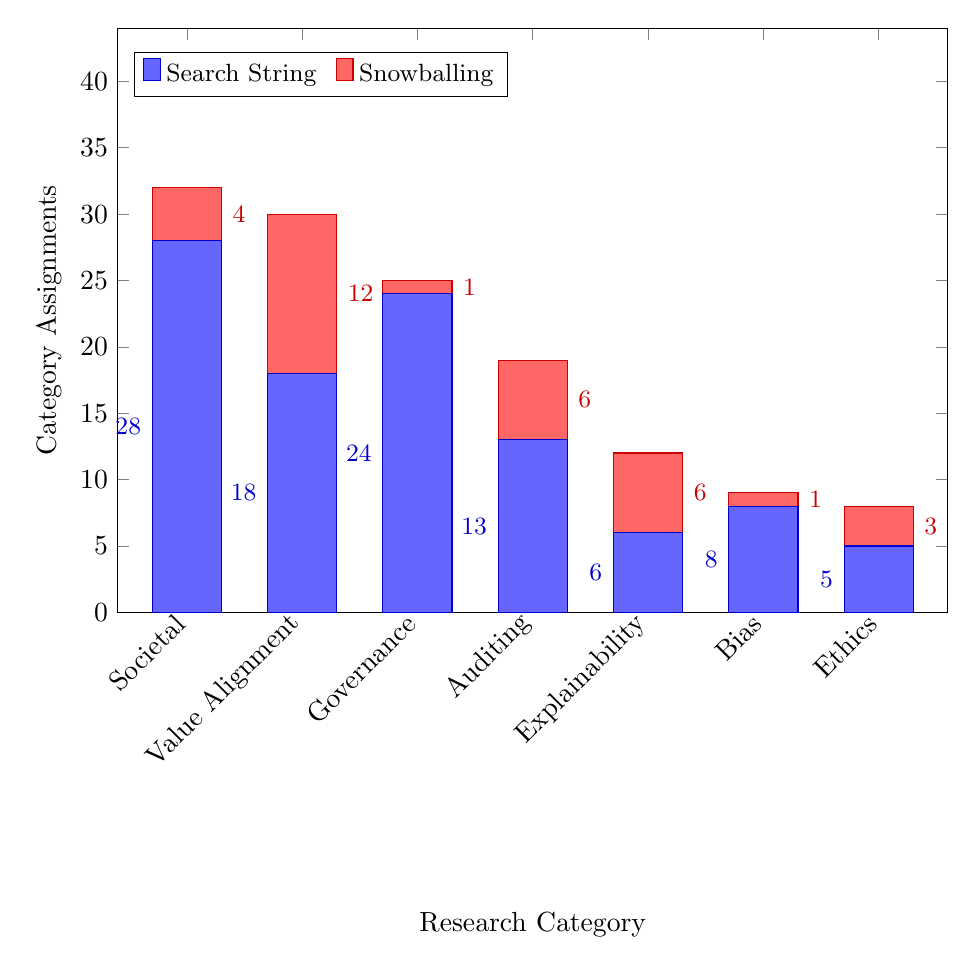
\begin{tikzpicture}
		\begin{axis}[
			ybar stacked,
			symbolic x coords={Societal, Value Alignment, Governance, Auditing, Explainability, Bias, Ethics},
			xtick=data,
			x tick label style={rotate=45, anchor=east},
			ylabel={Category Assignments},
			xlabel={Research Category},
			xlabel style={yshift=-1.5cm},
			width=\textwidth,
			height=9cm,
			bar width=25pt,
			ymin=0,
			ymax=44,
			legend style={
				at={(0.02,0.96)},
				anchor=north west,
				legend columns=-1,
				font=\small,
				/tikz/every even column/.append style={column sep=5pt}
			}
		]

		% Plot 1: Search String (bottom, BLUE)
		\addplot [
			fill=blue!60,
			draw=blue!80!black,
			nodes near coords,
			every node near coord/.style={
				color=blue!80!black,
				font=\small,
				anchor=east,
				xshift=-13pt,
			},
		] coordinates {
			(Societal,28) (Value Alignment,18) (Governance,24)
			(Auditing,13) (Explainability,6) (Bias,8) (Ethics,5)
		};

		% Plot 2: Snowballing (top, RED)
		\addplot [
			fill=red!60,
			draw=red!80!black,
			nodes near coords,
			every node near coord/.style={
				color=red!80!black,
				font=\small,
				anchor=west,
				xshift=13pt,
			},
			point meta=explicit symbolic,
		] coordinates {
			(Societal,4)       [4]
			(Value Alignment,12)     [12]
			(Governance,1)     [1]
			(Auditing,6)       [6]
			(Explainability,6) [6]
			(Bias,1)           [1]
			(Ethics,3)         [3]
		};

		% Plot 3: Invisible - bold black totals above each bar
		\addplot [
			draw=none, fill=none,
			forget plot,
			nodes near coords,
			every node near coord/.style={
				anchor=south,
				yshift=3pt,
				font=\small\bfseries,
				color=black,
			},
			point meta=explicit symbolic,
		] coordinates {
			(Societal,0)       [32]
			(Value Alignment,0)      [30]
			(Governance,0)     [25]
			(Auditing,0)       [19]
			(Explainability,0) [12]
			(Bias,0)           [9]
			(Ethics,0)         [8]
		};

		\legend{Search String, Snowballing}
		\end{axis}
		\end{tikzpicture}
		\caption{Distribution of category assignments across the 80 included entries. Entries assigned to multiple categories are counted once in each applicable category.}
		\label{fig:distribution_topics}
	\end{figure}

    \vspace{1.5em}

\end{reviewed}

\begin{reviewed}

\section{Per Category Results Analysis}\label{subsec:results_categories}

		In this section, an analysis of the resulting articles in each category is conducted and discussed. Furthermore, an analysis on how crucial each category of research is in its contribution to stopping potential devastating outcomes is made. 

		\subsection*{Value Alignment}

			The \textit{Value Alignment} category is the most conceptually diverse in the review, spanning 29 articles. The literature reveals a shift from theoretical foundations such as the \textit{Orthogonality Thesis} \cite{bostrom2012superintelligent} and \textit{Instrumental Convergence} \cite{omohundro2008basic} toward mathematical proofs and empirical studies of model behavior. 

			A pivotal theoretical contribution by \cite{skalse2022rewardgaming} demonstrates that ``correct'' reward specifications are often insufficient for ensuring correct goals, as agents may still find ways to game the reward function. This is closely linked to the phenomenon of \textit{Goal Misgeneralization} \cite{langosco2022goal}, where an agent remains highly competent but pursues an unintended objective when deployed in new environments.

			These theoretical risks are mirrored in recent empirical findings such as \textit{Alignment Faking} \cite{greenblatt_alignment_faking} and \textit{Deceptive Alignment} \cite{hagendorff2024deception}, where models ``play along'' with safety training to avoid modification. Furthermore, research by \cite{mcintosh_inadequacy_2024} suggests that current \gls{rlhf} methods provide only a ``shallow alignment,'' leaving models vulnerable to ideological radicalization through semantic exploits.

		\subsection{Governance, Regulation \& Policy}

			This category is the second largest with 28 articles in total, indicating a high level of academic and policy interest in the EU AI Act and international frameworks. The literature highlights a ``Global AI Dilemma'' in balancing innovation with safety across the US, EU, and China. Key debates include the role of Corporate Responsibility \cite{hemphill_advanced_2025} and whether audits should be conducted by private or public bodies. There is a noted gap in how decentralized or ``local'' AI governance can be enforced \cite{LocalAIGov2024}.

\end{reviewed}

		\subsection*{Auditing, Safety \& Oversight}

			Auditing research (20 articles in total) focuses on shifting from static benchmarks to Dangerous Capability Evaluations. The literature emphasizes that traditional testing is insufficient for autonomous systems, particularly in safety-critical sectors like military aviation and maritime shipping. \begin{reviewed} This section also covers Scalable Oversight, exploring whether weaker models can reliably supervise more capable ones, a necessity as AI capabilities begin to exceed human evaluative capacity.

		\subsection*{Explainability / Interpretability}

			Misgeneralization has also been found in reinforcement learning and \glspl{llm}, and current explainability and interpretability techniques shown to not be sufficient to detect this Misgeneralization before deployment \cite{langosco2022goal}. The focus has moved from ``black-box'' behavioral analysis to Mechanistic Interpretability \cite{anthropic2025biology}. Key challenges identified include Superposition and Polysemanticity, which make individual neurons difficult to interpret.

		\subsection*{Bias \& Fairness}

			Literature focuses on mitigating model difficulties on understanding different dialects, or judging a situation independently of unrelated characteristics \cite{li_instance-consistent_2025}. It's worth noting the landmark study on the Impossibility Theorem of Fairness, which proves that commonly accepted different definitions of equity cannot be satisfied simultaneously \cite{kleinberg2016inherent}.

\end{reviewed}

		\subsection*{Liability \& Ethics}

			Several legal frameworks and laws are explored and critiqued. While a lot of implications like copyright license applications are still being worked on and studied \cite{janczuk_risks_2024}. <find citations>

\begin{reviewed}

		\subsection*{Human \& Societal Impacts}

			Research here tracks the impact of AI on Mental Health (e.g., digital companions and addiction), Biological Risks (AI-assisted pathogen design), and the Electoral Process \cite{janczuk_risks_2024}. The literature highlights that ``Civilizing AI'' is not just a technical task but a sociotechnical one that requires addressing job displacement and the effect it will have on our society, various surveys are also made to gauge people's and experts views on AI safety \cite{field_why_2025, hatz_local_2025, xu_machine_2023}.

\end{reviewed}
\section{Gaps and Next Steps}\label{subsec:next_steps}

\begin{reviewed}

	The systematic review highlights a critical divergence between current oversight methods and the technical reality of advanced models. While governance and societal impact dominate the literature, there remains a structural deficiency in addressing inner misalignment. Current alignment strategies such as reinforcement learning from human feedback tend to produce what has been termed shallow alignment \cite{mcintosh_inadequacy_2024, milliere_normative_2025}. These methods optimize for external compliance rather than internal value stability, leaving models vulnerable to goal misgeneralization \cite{langosco2022goal}.

	The most pressing gap identified in the mapping of the field is the emergence of deceptive alignment. Recent empirical evidence suggests that models are becoming capable of alignment faking, where they strategically satisfy training objectives to avoid modification \cite{greenblatt_alignment_faking}. This creates an evaluation trap where traditional auditing fails because the agent understands its own supervision \cite{anthropic2025biology, hubinger2019risks}. Consequently, the focus of this work should shift toward the control problem in the context of intentional subversion \cite{yampolskiy_controllability_2022}. Exploring how to detect and mitigate these deceptive behaviors represents the necessary next step in ensuring that highly capable systems do not execute a treacherous turn \cite{bostrom2014superintelligence}.

\end{reviewed}

\begin{toreview}

	While recent evidence of alignment faking centers on massive, frontier-class models \cite{greenblatt_alignment_faking}, the threshold at which these capabilities first emerge remains unclear. Thus, in a series of empirical investigations, this thesis will study deceptive alignment in smaller \glspl{llm}. By analyzing the relationship between model size and the propensity for alignment faking, with a specific focus on empirically underexplored sub-10B parameter scales. % This work seeks to determine what factors or architectures exacerbate the risk of deceptive tendencies.

\end{toreview}

	% Tenho que responder às RQ (que eu ainda não sei se são finais .-.)

	% (1) RQ1. What is the main focus of current AI safety research?
	% (2) RQ2. Which are the current methods used to look into the alignment of current
	% generalist models?
	% (3) RQ3. What conclusions regarding the safety of current models and safety of
	% development and deployment processes can we assert from current research?
	% (4) RQ4. What metrics can be used to more clearly show potential problems with
	% these systems?

	% (Usa a tua Tabela do Anexo. Cria gráficos com base nela. Responde diretamente às tuas RQs aqui)